%% Paper 1 in the OUP authoring template (oup-authoring-template.cls, TeX Live 2026).
%% Layout and front matter follow OUP methodology-review conventions: title page, short abstract,
%% up to six keywords, up to five Key Points, statements and author biographies. No journal is implied.
%%
%% body.tex and supplementary.tex are generated from ../review_manuscript_draft.md by
%% scripts/build_manuscript_latex.py; references.bib by scripts/build_manuscript_references.py.
%% Edit the Markdown master, not body.tex. Front and back matter are edited here.
%% Build: latexmk -pdf main.tex   (or: pdflatex, bibtex, pdflatex, pdflatex)

% Numbered citations. The class option "numbered" is not used: it switches the class's forced-numbers
% fallback off, and citations of a numeric .bst then print empty.
\PassOptionsToPackage{numbers,square,sort&compress}{natbib}
\documentclass[webpdf,contemporary,large]{oup-authoring-template}

\usepackage{tabularx}
\usepackage{xurl}
\usepackage{draftwatermark}
\SetWatermarkText{Draft}
\SetWatermarkScale{1}
\SetWatermarkLightness{0.93}

\graphicspath{{figures/}}
\providecommand{\tightlist}{\setlength{\itemsep}{0pt}\setlength{\parskip}{0pt}}
\newcommand{\citeplaceholder}[1]{\textcolor{red}{[#1]}}
\newcommand{\draftnote}[1]{\textcolor{red}{#1}}
\newcommand{\todo}[1]{\textcolor{red}{[#1]}}

\begin{document}

\journaltitle{Manuscript draft}
\DOI{}
\copyrightyear{2026}
\pubyear{2026}
\access{Draft of 15 October 2026 (manuscript v0.5.1); not peer reviewed}
\appnotes{Review}

\firstpage{1}

\title[Translate or encode? Text--omics foundation models]{Translate or encode? Two design cultures for coupling language and omics data in generative foundation models: a scoping review}

\author[1,$\ast$]{Bogdan Didenko}
\author[2]{\todo{Co-author names, affiliations and ORCID iDs}}

\address[1]{\orgdiv{\todo{Department}}, \orgname{Lviv Polytechnic National University}, \orgaddress{\state{Lviv}, \country{Ukraine}}}
\address[2]{\orgdiv{\todo{Department}}, \orgname{\todo{Organization}}, \orgaddress{\country{\todo{Country}}}}

\corresp[$\ast$]{Corresponding author: Bogdan Didenko, \todo{e-mail, telephone}}

\abstract{Generative foundation models that combine natural language with omics data must decide how biology reaches the language model: by translating it into the model's own tokens or by encoding it with a biological model and injecting the result. This PRISMA-ScR scoping review (searches to 9 August 2026) includes 55 records: 51 independent works, 109 models and 585 input routes. Routes were decomposed into a library of 22 data operations, and a targeted pass charted rationales, supervision, dependence tests and cross-representation comparisons. Seventeen works are token-native, 16 encoder-mediated and 8 hybrid, and 9 use language to condition a biology model. Token-native works keep a median of 100 gene names per cell, and only 2 of the 51 works write measured values as numbers. Works that inject encoder outputs give the language model 1--256 vectors per biological object, and a third of the route steps in the median encoder-mediated work are opaque learned modules. Twenty-five works train or evaluate on text written by another LLM, and only 22 test whether outputs depend on the biological input. In 31 cross-culture comparisons in 20 works, the authors' own representation won 28. Opponents were mostly released, unadapted forms of the other culture, and opponents trained by the proposing team lost all 11 comparisons. The two cultures keep complementary parts of biological data, and the published comparisons cannot yet tell which serves a given task better. We propose a neutral comparison protocol and a reporting card for input representations.}

\keywords{large language models, foundation models, single-cell transcriptomics, multimodal learning, input representation, scoping review}

\maketitle

% Generated by scripts/build_manuscript_latex.py from manuscript/review_manuscript_draft.md; do not edit.




\section{Introduction}

Large language models are being extended to biological data: single-cell profiles, nucleotide and protein sequences, histology and microscopy images, molecular graphs and knowledge bases \citeplaceholder{CITE}. Every such system has to decide how a measurement reaches a network trained on text. Two answers recur (Figure 1a).

\begin{figure*}[!t]
\centering
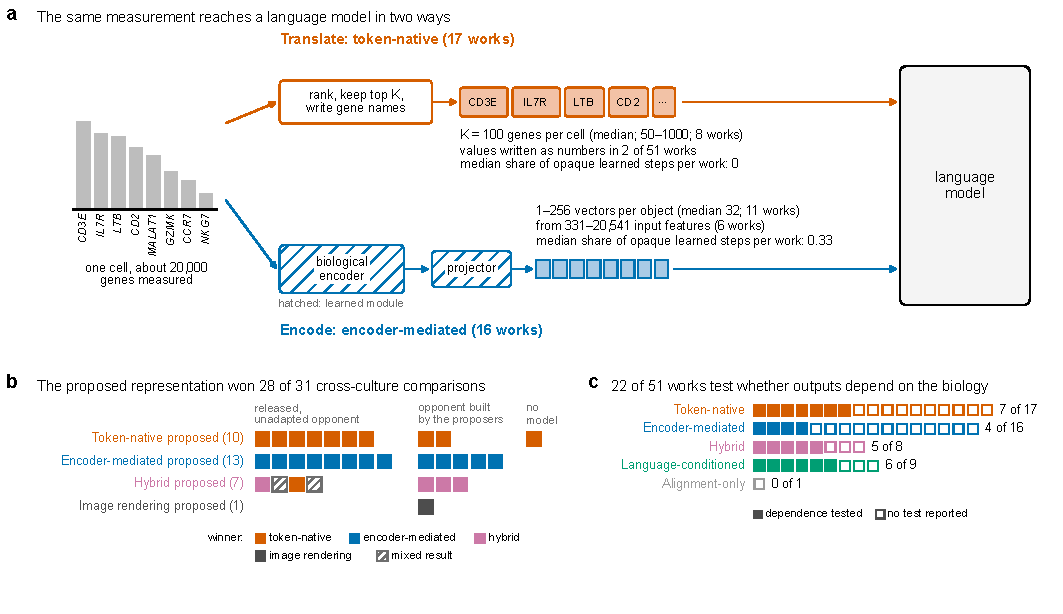
\includegraphics[width=\textwidth]{figure1.pdf}
\caption{\textbf{Two ways to give a language model a measurement, and why the published evidence cannot choose between them.} (a) The two design cultures, annotated with corpus values. Token-native works rank a cell's genes, keep the top K and write their names into the language model's token stream (K stated in 8 works: 5 token-native, 3 hybrid). Encoder-mediated works pass the measurement through a biological encoder and a projector and inject a few vectors per object (stated in 11 works across cultures; input feature counts in 6). Opaque-step shares are medians over works of the share of biological route steps that are learned modules left unexpanded (14 token-native and 14 encoder-mediated works with decomposed biological routes). Gene names and bar heights are illustrative. Hybrids (8 works) use both lanes; 9 works condition a biology generator on language, and 1 aligns modalities without a generative host. (b) The 31 cross-culture comparison units in 20 works, one square per unit, by the culture of the proposed representation (rows) and how the opponent was obtained (columns). Colour shows the winning culture; hatching marks a mixed result. Released, unadapted opponents are prompted general LLMs and released encoder models used frozen or as published; opponents built by the proposers are baselines or ablations trained on the same data. Image rendering is OpticalDNA's DNA-as-image arm. (c) Works reporting any test of whether outputs depend on the biological input (removal, mismatch or shuffling, random input, a no-biology baseline, content perturbation), one square per work.}\label{fig:1}
\end{figure*}

\begin{itemize}
\item \textbf{Translate:} the measurement is written in the language model's own tokens. Examples are a ranked list of gene names, a nucleotide string, or a vocabulary extended with biological symbols. The model needs no new components and can draw on what it learned about named entities during pretraining.
\item \textbf{Encode:} the measurement is passed through a biological encoder, and the resulting vectors are injected into the language model as soft tokens, through cross-attention or as conditioning. This can keep magnitudes and structure, but the transformation is learned and opaque.
\end{itemize}

We call these choices design cultures. Each comes with its own conventions for what is kept, what is trained, how outputs are supervised and how claims are tested.

Existing reviews organise text–biology models by architecture family, biological domain or task \citeplaceholder{CITE; see \nolinkurl{data/existing_reviews_compilation.md}}. Individual papers argue for one culture and against the other \citeplaceholder{CITE}. We are not aware of a cross-paper, evidence-grounded account that asks four things:

\begin{itemize}
\item what each culture keeps of the data;
\item how each justifies itself;
\item how each is supervised and tested;
\item whether the published comparisons between them can tell which serves a given task better.
\end{itemize}

This review answers these questions for generative foundation models that couple text with omics data. Text models of protein sequences, protein structures or small molecules are an adjacent family that this review's search did not target (\S{}2.2, \S{}5). It rests on:

\begin{enumerate}
\item a reproducible living search and screening pipeline;
\item a route-level charting of every model's inputs;
\item an operation-level decomposition of each input path into reusable data operations (library release 1.3.0);
\item a targeted charting pass of design rationales, adaptation, LLM-generated supervision, biology-dependence tests and cross-representation comparisons.
\end{enumerate}


\section{Methods}


\subsection{Protocol and reporting}

Reported following PRISMA-ScR~\cite{prisma_scr}, with PRISMA-S~\cite{prisma_s} for the search and PRISMA-trAIce-style reporting of LLM-assisted steps. The protocol (\nolinkurl{protocol/PRISMA_protocol.md}, v4.5, 2026-08-09) was not registered. Amendments are logged in the protocol's amendment section.


\subsection{Eligibility}

Included records describe a generative model with foundation-model characteristics that combines a text modality (natural language, or gene tokens processed in a generative language-model style) with at least one biological data modality, published 2018–2026, in English and open access. Exclusions: no biological modality (EC1), no text component or no substantive text–biology bridge (EC2), encoder-only or non-generative (EC3), no foundation-model component (EC4), non-computational (EC5), non-scholarly (EC6), reviews (EC7), duplicates (EC8). Full criteria: \nolinkurl{protocol/eligibility_criteria.md}.

\textbf{Scope boundary.} Biological data were defined as omics data: single-cell and bulk transcriptomic, chromatin-accessibility, surface-protein, spatial, methylation, epigenomic, genomic and other omics profiles (proteomics, metabolomics). The search vocabulary followed this definition (\S{}2.3) and has no molecule-level terms such as protein, amino acid, DNA or nucleotide. Models whose biological input is a protein or nucleotide sequence were therefore retrieved only when their records also used omics terms. Thirteen included records carry protein inputs (sequences, structures, interaction networks or knowledge bases). Ten of them combine proteins with transcriptomic, nucleotide, methylation or perturbation data. In three, proteins (with small molecules in BioMedGPT~\cite{biomedgpt}) are the only biological input: Chroma~\cite{chroma}, PROCYON~\cite{procyon} and BioMedGPT. These three entered through an omics term in the abstract (PROCYON), through Google Scholar (BioMedGPT) or through Scopus, which also searches indexed keywords (Chroma), and are kept as screened.


\subsection{Information sources and search}

Three concept blocks (biological data AND text/language AND foundation-model/generativity) were adapted per database (\nolinkurl{protocol/queries/}). The biological-data block lists omics and single-cell terms (for example single-cell, RNA-seq, gene expression, chromatin accessibility, spatial transcriptomics, transcriptomics, genomics, proteomics, epigenomics) and no molecule-level terms. Supplementary Table S0 lists, for each round and database, the interface, execution date, date and other limits as executed, and the records returned and retained. Supplementary Text S1 gives every query string as executed.

\begin{itemize}
\item \textbf{Sources.} Rounds 1–4 searched seven sources:
\begin{itemize}
\item PubMed (NCBI E-utilities);
\item Scopus (Scopus Search API);
\item Semantic Scholar (bulk search API);
\item arXiv (arXiv API; categories cs.LG, cs.AI, cs.CL, q-bio.GN, q-bio.QM and stat.ML);
\item bioRxiv and medRxiv preprints through Europe PMC (REST API, SRC:PPR);
\item Springer Nature (Meta and Open Access APIs);
\item Google Scholar (\texttt{scholarly} Python library).
\end{itemize}
Round 5 added OpenAlex and queried Google Scholar with one combined query through a provider export (SerpAPI).
\item \textbf{Rounds.} The baseline (window 2018-01-01 to 2026-02-28) was executed on 2026-02-15 under protocol v3.1. Before screening, it replaced a v3.0 execution of 2026-02-06. Four top-ups covered 2026-03-01 to 04-14, 04-15 to 06-10, 06-11 to 07-06 and 07-07 to 08-09. Each was executed on the last day of its window, except the August round (executed 2026-08-10). The five rounds retained 5,534, 867, 933, 197 and 639 records (8,170).
\item \textbf{Dates as executed.}
\begin{itemize}
\item Exact dates in the query: PubMed, arXiv, Europe PMC, Springer Nature and OpenAlex.
\item Year in the query, then removal by exact date: Scopus and Semantic Scholar. Records removed (Scopus/Semantic Scholar): 18/1 in the baseline, then 165/226, 292/462, 389/766 and 485/914 in the top-ups. In round 5, 39 Semantic Scholar records without a publication date were kept.
\item Year only: Google Scholar.
\end{itemize}
The baseline ran on 2026-02-15, so no date-bounded query covered records dated 2026-02-16 to 2026-02-28 (\S{}5).
\item \textbf{Other limits.}
\begin{itemize}
\item PubMed: English[Language] and ``free full text''[sb].
\item Scopus: LANGUAGE(English) and OPENACCESS(1).
\item OpenAlex: language en and is\_oa.
\item Semantic Scholar, arXiv, Europe PMC and Google Scholar: no language or access limit.
\end{itemize}
Where no limit was applied at search, English and open access were enforced at screening and full-text retrieval. No published search filters were used.
\item \textbf{Springer Nature.} The free API searches full text and cannot be restricted to title and abstract. Retrieved records were therefore kept only if a term from each concept block appeared in the title or abstract. Raw to validated, by round: 17,130 to 272, 1,185 to 33, 1,129 to 27, 510 to 20 and 691 to 27. The flow counts the validated records.
\item \textbf{Google Scholar completeness.} The April and June rounds were rate-limited after 5 of 7 queries, and the July round returned no records. The baseline completion log was overwritten by a later Springer Nature-only rerun; the retained baseline records are preserved.
\item \textbf{Other methods.} No study registries, citation searching or contact with authors were used. One eligible record (XunZi~\cite{xunzi}) was recovered after a correction of the pre-screen lexical validator (\S{}3.1). The search strategy was not peer reviewed (for example with PRESS~\cite{press}).
\end{itemize}


\subsection{Deduplication and abstract enrichment}

Conservative exact matching (DOI, PMID, arXiv ID, normalised title), cross-round matching against the cumulative master, and a Crossref audit for hidden duplicates. Missing abstracts were enriched from Semantic Scholar, Crossref and PubMed; records still lacking an abstract were removed before screening.


\subsection{Screening}

Title/abstract screening applied the eligibility decision tree with two role-separated LLM reviewers (scope and architecture) and an adjudicator for conflicts (Codex CLI, \nolinkurl{gpt-5.4-mini}; prompts and schemas hash-pinned). Full-text screening used Docling~\cite{docling} conversions; Docling Graph provenance reconstructed the complete data-source and input-representation sections, which were screened with the title and abstract. Records still uncertain after adjudication were resolved by the review lead from the full sections, keeping the automated decision alongside. The roles are prompts executed by the same model, not independent human reviewers. Run-to-run stability of this screening is reported in a companion methods paper \citeplaceholder{CITE companion manuscript}.


\subsection{Data charting: input routes and taxonomy}

The unit of charting is a grounded input route: one source object carried through its transformation chain to the model-visible carrier. Routes were extracted from the full text with three frozen direct runs plus dense-coverage candidates, and classified by carrier mechanism into five families and 15 subtypes (\nolinkurl{input-representation-taxonomy-v1}). Biological modality, lifecycle phase, text role and fusion topology were charted as orthogonal dimensions. Agreement across the three runs on the 55-record corpus: route Jaccard 0.945–0.969; carrier-family exact agreement 0.929; Krippendorff's alpha 0.881 (acceptance thresholds 0.80, 0.90, 0.80). Dated author-led amendments are recorded in the atlas metadata.


\subsection{Operation-level decomposition}

Each documented input path is reconstructed as a directed graph of calls to a library of 22 reusable operations (normalisation, log transform, binning, tokenisation, table lookup, projection, concatenation, attention and others) with named ports and instance parameters (\nolinkurl{protocol/REPRESENTATION_LIBRARY_GUIDE.md}; catalog definitions of release 1.3.0). Steps whose internal computation the paper does not state remain unexpanded boundaries. A four-paper pilot (ChatNT~\cite{chatnt}, InstructCell~\cite{instructcell}, X-Cell~\cite{xcell}, MUPAD~\cite{mupad}; 47 trajectories, 509 operation calls) was curated by the authors. The remaining 50 papers were decomposed by agents (Codex CLI, \nolinkurl{gpt-5.6-luna}, reasoning effort high; the earlier \nolinkurl{gpt-5.4-mini} is no longer available through Codex) under protocol v3.2 (\nolinkurl{scripts/operation_decomposition_v3.py}; v3.2 sharpens the boundaries between align, concatenate and serialize, and partition and select, after run-to-run disagreements under v3.1; \nolinkurl{analysis/representation_block_library_2026-10-04/DECISION_MEMO_1.3.0.md}). The structure is fixed by the charted routes: one trajectory per charted configuration and one step per element of each route's verbatim transformation chain. For each step the agent returns only a decision, a closed category plus the library operation(s) named in the element text, with stated parameter values, verbatim evidence and the echoed chain element. A predefined rule set decides the category (e.g.\ unexpanded learned module, data provenance, external text generator, unspecified fusion). Routes without a recorded chain get a mechanical decision. Nodes, ports and data flow are compiled from these decisions, and the result is checked mechanically for verbatim evidence, catalog ports and declared parameters. The full paper text is supplied without truncation. Each paper was decomposed in three independent runs (up to four mechanical repairs each), and the published decision per step is the majority label. Steps without a majority remain unresolved boundaries and are listed for the library steward, as are steps decided 2 of 3. A separate parameter pass then read the whole paper again, with the operations fixed. For every declared parameter of every library call (2,433 slots in 1.3.0; definitions in \nolinkurl{protocol/OPERATION_PARAMETER_GLOSSARY.md}) it decided whether the paper states the value for that data path, with verbatim evidence checked mechanically. Values that only follow from convention, released code or cited papers do not count. This pass also used three runs per paper and the majority status; its rules were tuned on the ten development papers (two iterations) and then frozen. Before the first run we fixed its gate: on ten held-out papers, consensus status agreement between runs 1-3 and 4-6 of at least 0.90 (\nolinkurl{analysis/operation_decomposition_v31_2026-10-12/parameter_pass/GATE.md}). The result was library release 1.2.1. Under v3.2, 39 of 1,468 steps changed operation; the parameter pass was repeated for the 16 affected papers (three runs), and slots of unchanged calls were carried over. The result is library release 1.3.0. No reviewer-agent pass was run on it. The protocol was developed iteratively on ten length-stratified papers and evaluated on held-out papers with the rules frozen. Stability was measured as agreement between the consensus of runs 1-3 and of runs 4-6 against a predeclared gate (\nolinkurl{analysis/operation_decomposition_2026-10-07/stabilization/GATE.md}, \nolinkurl{STABILIZATION_REPORT.md}). The withdrawn OKR-Cell~\cite{okrcell} preprint is not included.


\subsection{Synthesis}

Descriptive counts of models per family, subtype, fusion topology, text role and lifecycle phase (a model is counted once per value it carries), records per publication year, operation reuse measured as distinct papers per operation, and the share of operation calls whose declared parameters the paper leaves unstated.


\subsection{Motifs and design-pattern taxonomy}

Model-level paths. For each model configuration, the decomposed routes (agent papers) or the author-curated graphs (pilot papers, all root-to-model paths) were turned into paths of role-aware operation tokens. Provenance and identity steps were dropped and repeated identical operations collapsed. Each operation's role follows from its inputs: biological only, text only, or joining biological and text inputs. Unexpanded learned modules were kept as typed tokens (\nolinkurl{scripts/build_model_graphs.py}).

Motifs. Closed frequent sub-chains (contiguous and gapped) were mined at the operation and family levels, with support counted in papers (at least 4 papers; no length limit; \nolinkurl{scripts/mine_subchains.py}). Supported, interpretable sub-chains were named as motifs with templates, members, parameter reporting and evidence-quoted examples (\nolinkurl{analysis/motif_library_2026-10-14/MOTIF_LIBRARY.md}, \nolinkurl{scripts/build_motif_library.py}). Stability: mining was repeated on each single decomposition run.

Design axes. Each route was also coded on five axes along one canonical pipeline (source, curation, value transformation, carrier formation, interface): A1 carrier formation, A2 interface to the language model, A3 transformation of measured values (order only, discretised, learned compression, verbatim; with subset and normalisation modifiers), A4 text role and A5 transparency. Coding rules are deterministic over the chains and the charted atlas labels (\nolinkurl{analysis/design_taxonomy_2026-10-13/TAXONOMY_SPEC.md}). We tested coverage, independence (normalised mutual information) and robustness to decomposition runs. Archetypes are carrier x interface combinations; a model can carry several. An earlier version of this analysis compared exact route chains and reported no recurring recipes. That result was an artefact of chain construction (uneven wording granularity, non-computational steps counted as operations, fragmentary routes) and is withdrawn.


\subsection{Design cultures}

Each included work was assigned to one design culture by how biological data reach the generative model of its proposed system. Comparators, data-generation models and components are excluded from this assignment. The cultures are:

\begin{itemize}
\item \textbf{Token-native (T):} biology reaches a text-pretrained language model only as tokens in its own stream (natural-language names, sequence letters, or new symbolic tokens).
\item \textbf{Encoder-mediated (E):} biology reaches a text-pretrained language model only as continuous vectors from a biological encoder (soft tokens, attention bridges, conditioning).
\item \textbf{Hybrid (H):} the same system uses both channels.
\item \textbf{Language-conditioned biology model (C):} the generative host is a biology model and language enters as conditioning.
\item \textbf{Alignment-only (A):} no generative host.
\end{itemize}

The assignment uses the route archetypes of \S{}2.9 and the language-model backbones charted in \S{}2.11. It was made by the steward, and the decisions and notes are in \nolinkurl{analysis/design_culture_charting_2026-10-14/v11/steward_adjudication.json}. Reports of the same study were linked, so all culture-level counts are per independent work (51 works; Cell2Text~\cite{cell2text,cell2text_thesis}, CellWhisperer~\cite{cellwhisperer_preprint,cellwhisperer} and OmniNA~\cite{omnina_preprint,omnina} each have two reports).


\subsection{Targeted charting of rationale, supervision, testing and comparisons}

After the shortlist of candidate findings, a targeted charting pass was run with the author's approval (protocol \nolinkurl{design-culture-charting-v1.1}; \nolinkurl{scripts/run_design_culture_charting.py}). Each of the 54 records was charted in two independent agent runs (Codex CLI, \nolinkurl{gpt-5.6-luna}, reasoning effort high). Each run received the complete paper text and the atlas model list with model roles, and returned:

\begin{itemize}
\item \textbf{representation comparisons:} the arms with their category, the kind and design of the comparison, the task, the metric, the better arm and the stated numbers;
\item \textbf{tests of whether outputs depend on the biological input:} removal, mismatch or shuffling, random input, a no-biology baseline, or content, order or value perturbation, each with the reported result;
\item \textbf{evaluation formats} and \textbf{outputs};
\item \textbf{adaptation:} language-model backbones with size and training state, vocabulary extension, biological encoders and their state, and connectors;
\item \textbf{LLM-generated text} used for training or evaluation, with the generator, version, prompt and decoding disclosure, and verification;
\item \textbf{stated rationales} for or against an input representation.
\end{itemize}

Every item required verbatim evidence. Quotes were checked mechanically against the paper, with up to three repairs per run; all 108 runs passed validation. One quote broken by PDF line numbers was corrected by the steward. Agreement between runs is reported per field (\nolinkurl{analysis/design_culture_charting_2026-10-14/v11/agreement.json}).

The steward adjudicated the variables used for culture-level claims by reading the evidence:

\begin{itemize}
\item rationale items;
\item single-run dependence tests;
\item the cross-representation comparison units.
\end{itemize}

A comparison unit is one comparison between arms of different cultures, per work and task family, with the two runs merged. Each unit records:

\begin{itemize}
\item its design (a controlled ablation within one system; the authors' system against the same backbone given the data as text; or different systems);
\item the arm proposed by the authors;
\item the winning culture;
\item how the opponent arm was obtained: a prompted general LLM, an external frozen embedding or pretrained model, a trained baseline, a trained ablation, or a representation compared without a model.
\end{itemize}

For analysis, prompted general LLMs and external embeddings or pretrained models are grouped as released opponents, and trained baselines and ablations as opponents trained by the proposing team. Because units are nested in works, the comparison result is also counted per work (sign test). Contrasts between cultures use two-sided Fisher exact tests; they are exploratory and not adjusted for multiple comparisons.

The decisions are in \nolinkurl{comparison_units_adjudicated.csv} and \nolinkurl{steward_adjudication.json}. The numbers are computed by \nolinkurl{scripts/build_design_culture_synthesis.py}.


\section{Results}


\subsection{Study selection (Figure 2a, Supplementary Figure S1)}

The searches identified 8,170 records. After removing 3,083 duplicates and 225 records without a usable abstract, 4,862 were screened on title and abstract, and 4,599 were excluded. One post-screen duplicate was removed. Of 262 reports sought, 15 could not be retrieved and 14 lacked a valid targeted section pair, so 233 reports were assessed. 179 were excluded: no natural-language text component (131), application wrapper around an existing model (23), not generative (13), review or editorial (5), no biological modality (3), benchmark or resource without a new model (2), no foundation-model evidence (1), and no substantive text–biology bridge (1). Fifty-four records were included from the databases. One more (XunZi) was recovered when the pre-screen lexical validator was corrected and was screened with the same frozen pipelines, giving 55 records from 54 studies~\cite{alter,bioblip,biogpt_genomics,biomedgpt,bioreason,bioverse,c2sscale,calmflow,precious3gpt,cello1,cell2text_thesis,cell2text,cellhermes,chatcell,chatnt,chroma,okrcell,gemgen,balanced_finetuning,geneverse,human_genome_book,genna,genolator,gpgpt,cell2sentence,cellwhisperer_preprint,cellwhisperer,h2o,instructcell,leonine,scmmgpt,longevity_llm,medpalmm,mupad,teampath,ocellus,omicslm,omnidna,omnigene4,omnina_preprint,omnina,opticaldna,procyon,posttraining_bioreasoning,rvqalpha,scdiff,scicoreomics,scmir,scmoba,shusi,tissuenarrator,xcell,xunzi,celltosg2sequence,tissuecraftai}.

\begin{figure*}[!t]
\centering
\begin{minipage}[c]{0.34\textwidth}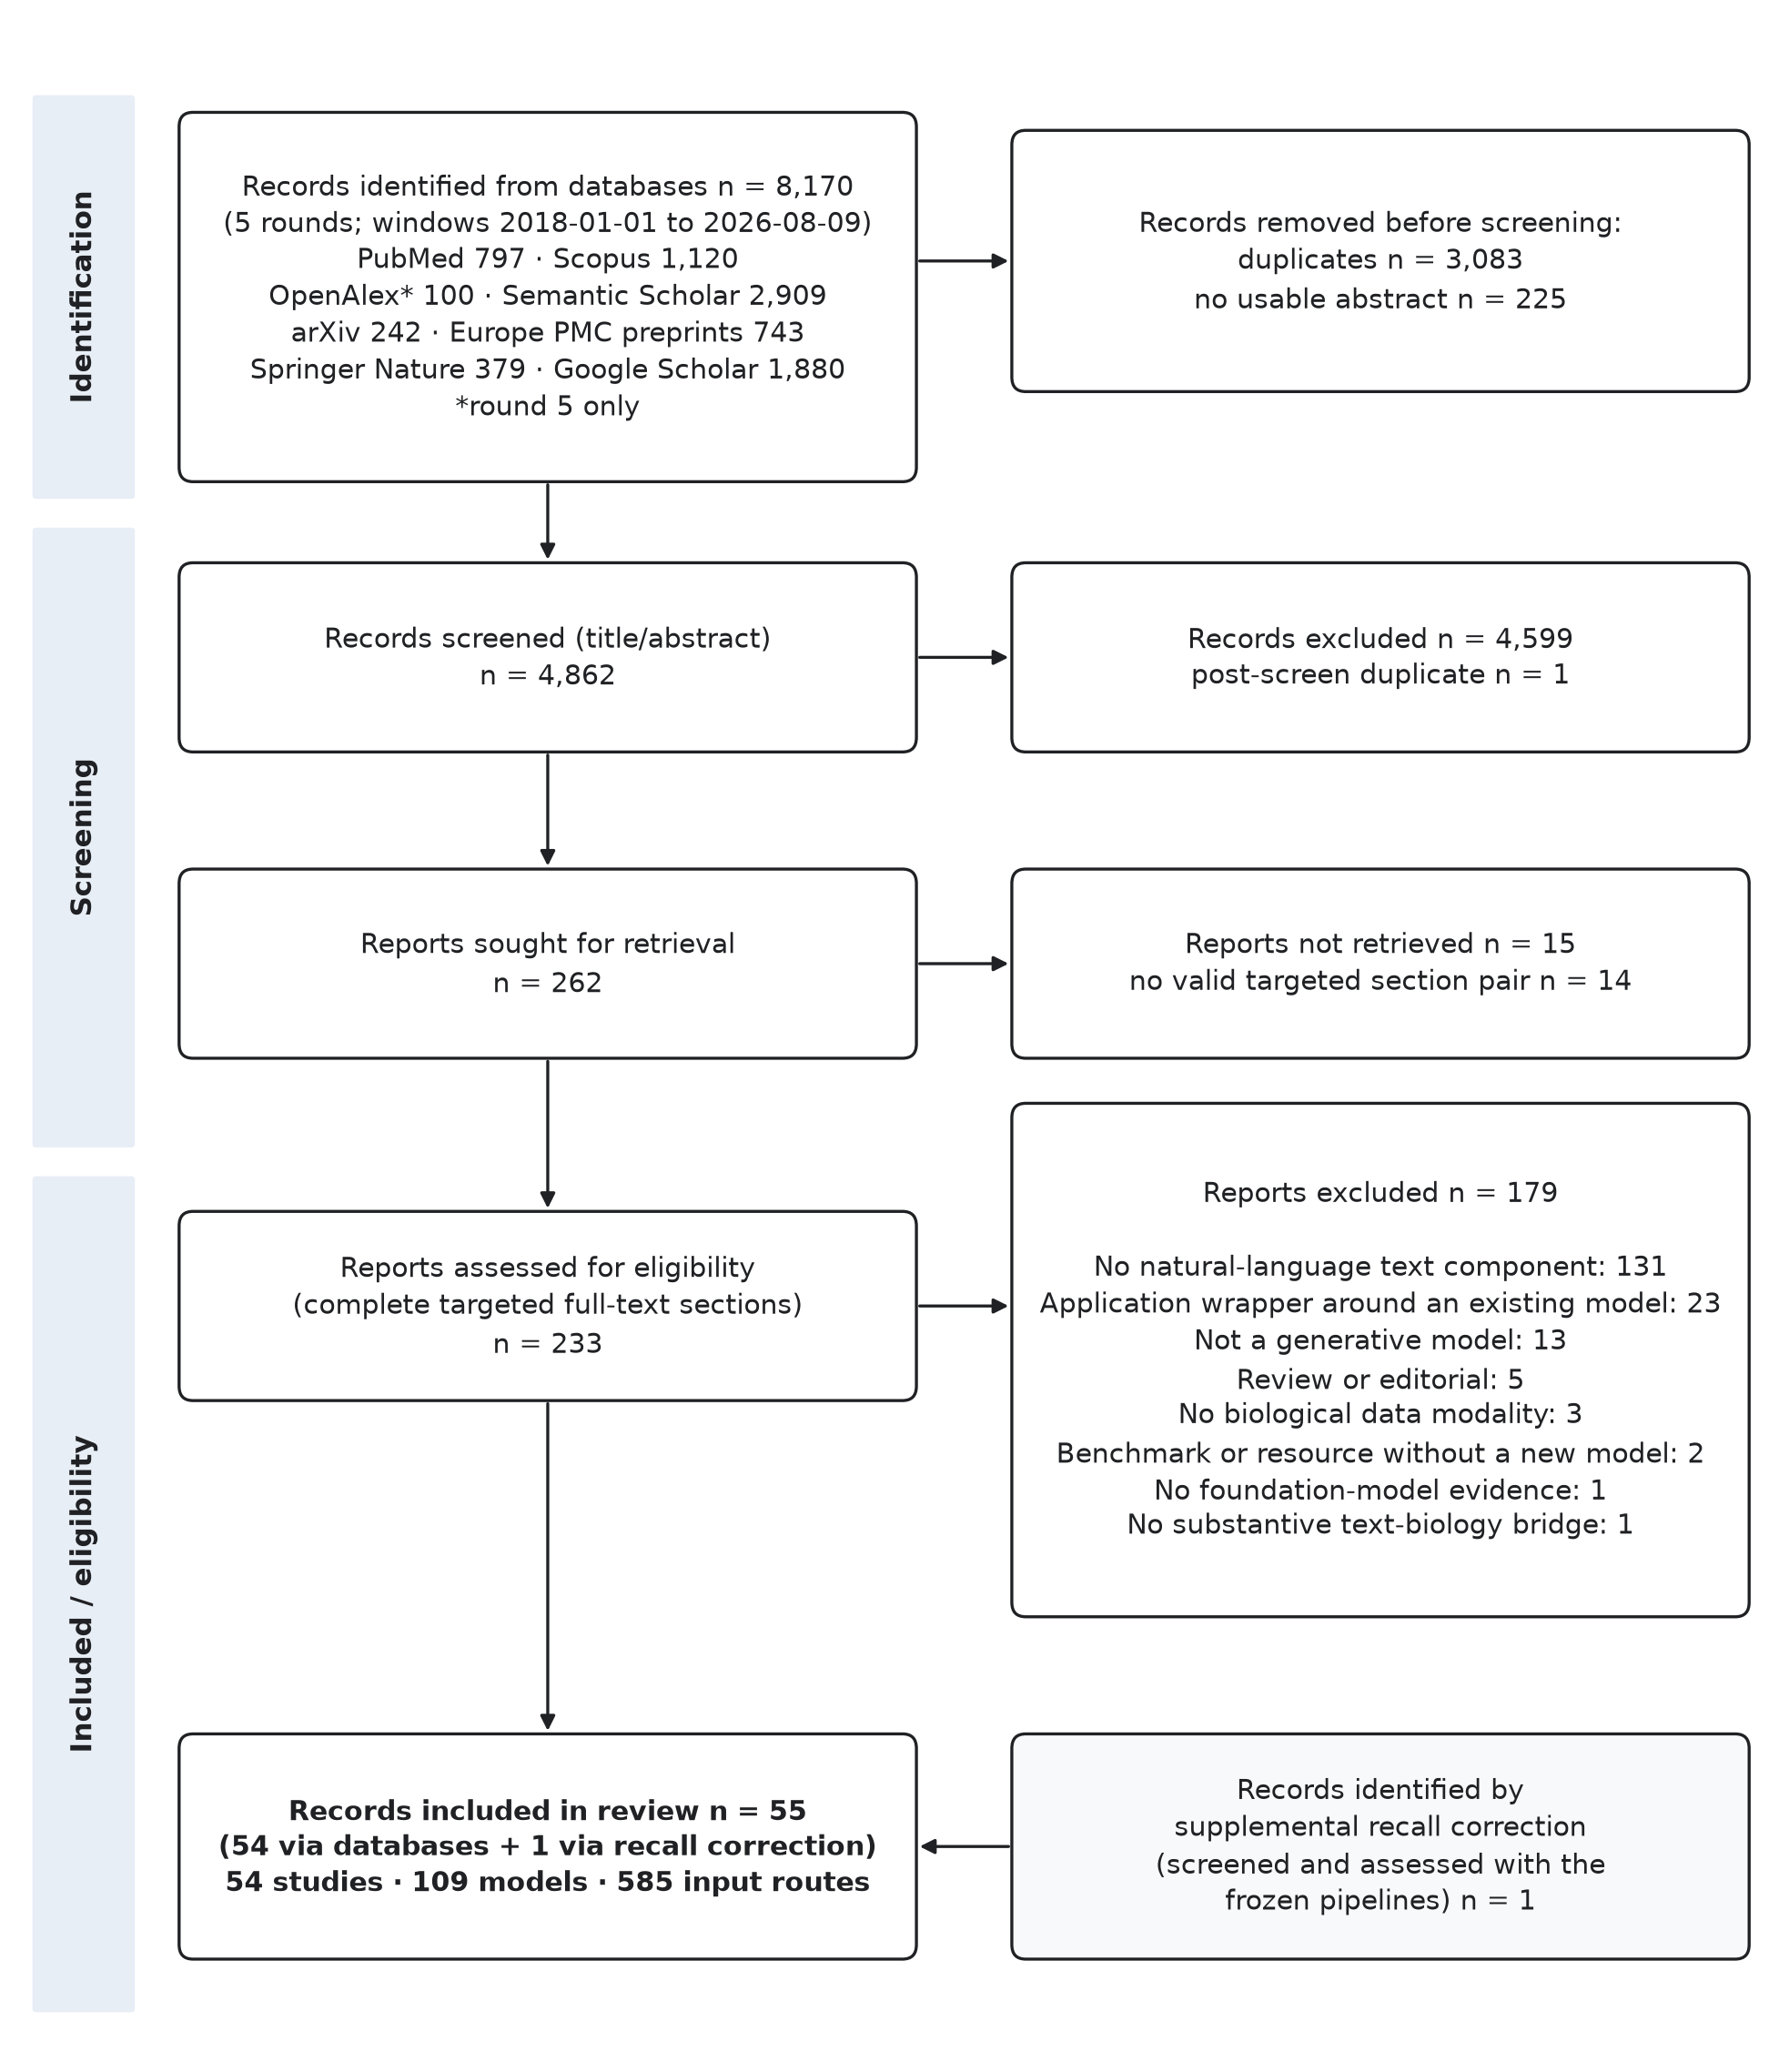
\includegraphics[width=\linewidth]{prisma_flow.png}\end{minipage}\hfill
\begin{minipage}[c]{0.63\textwidth}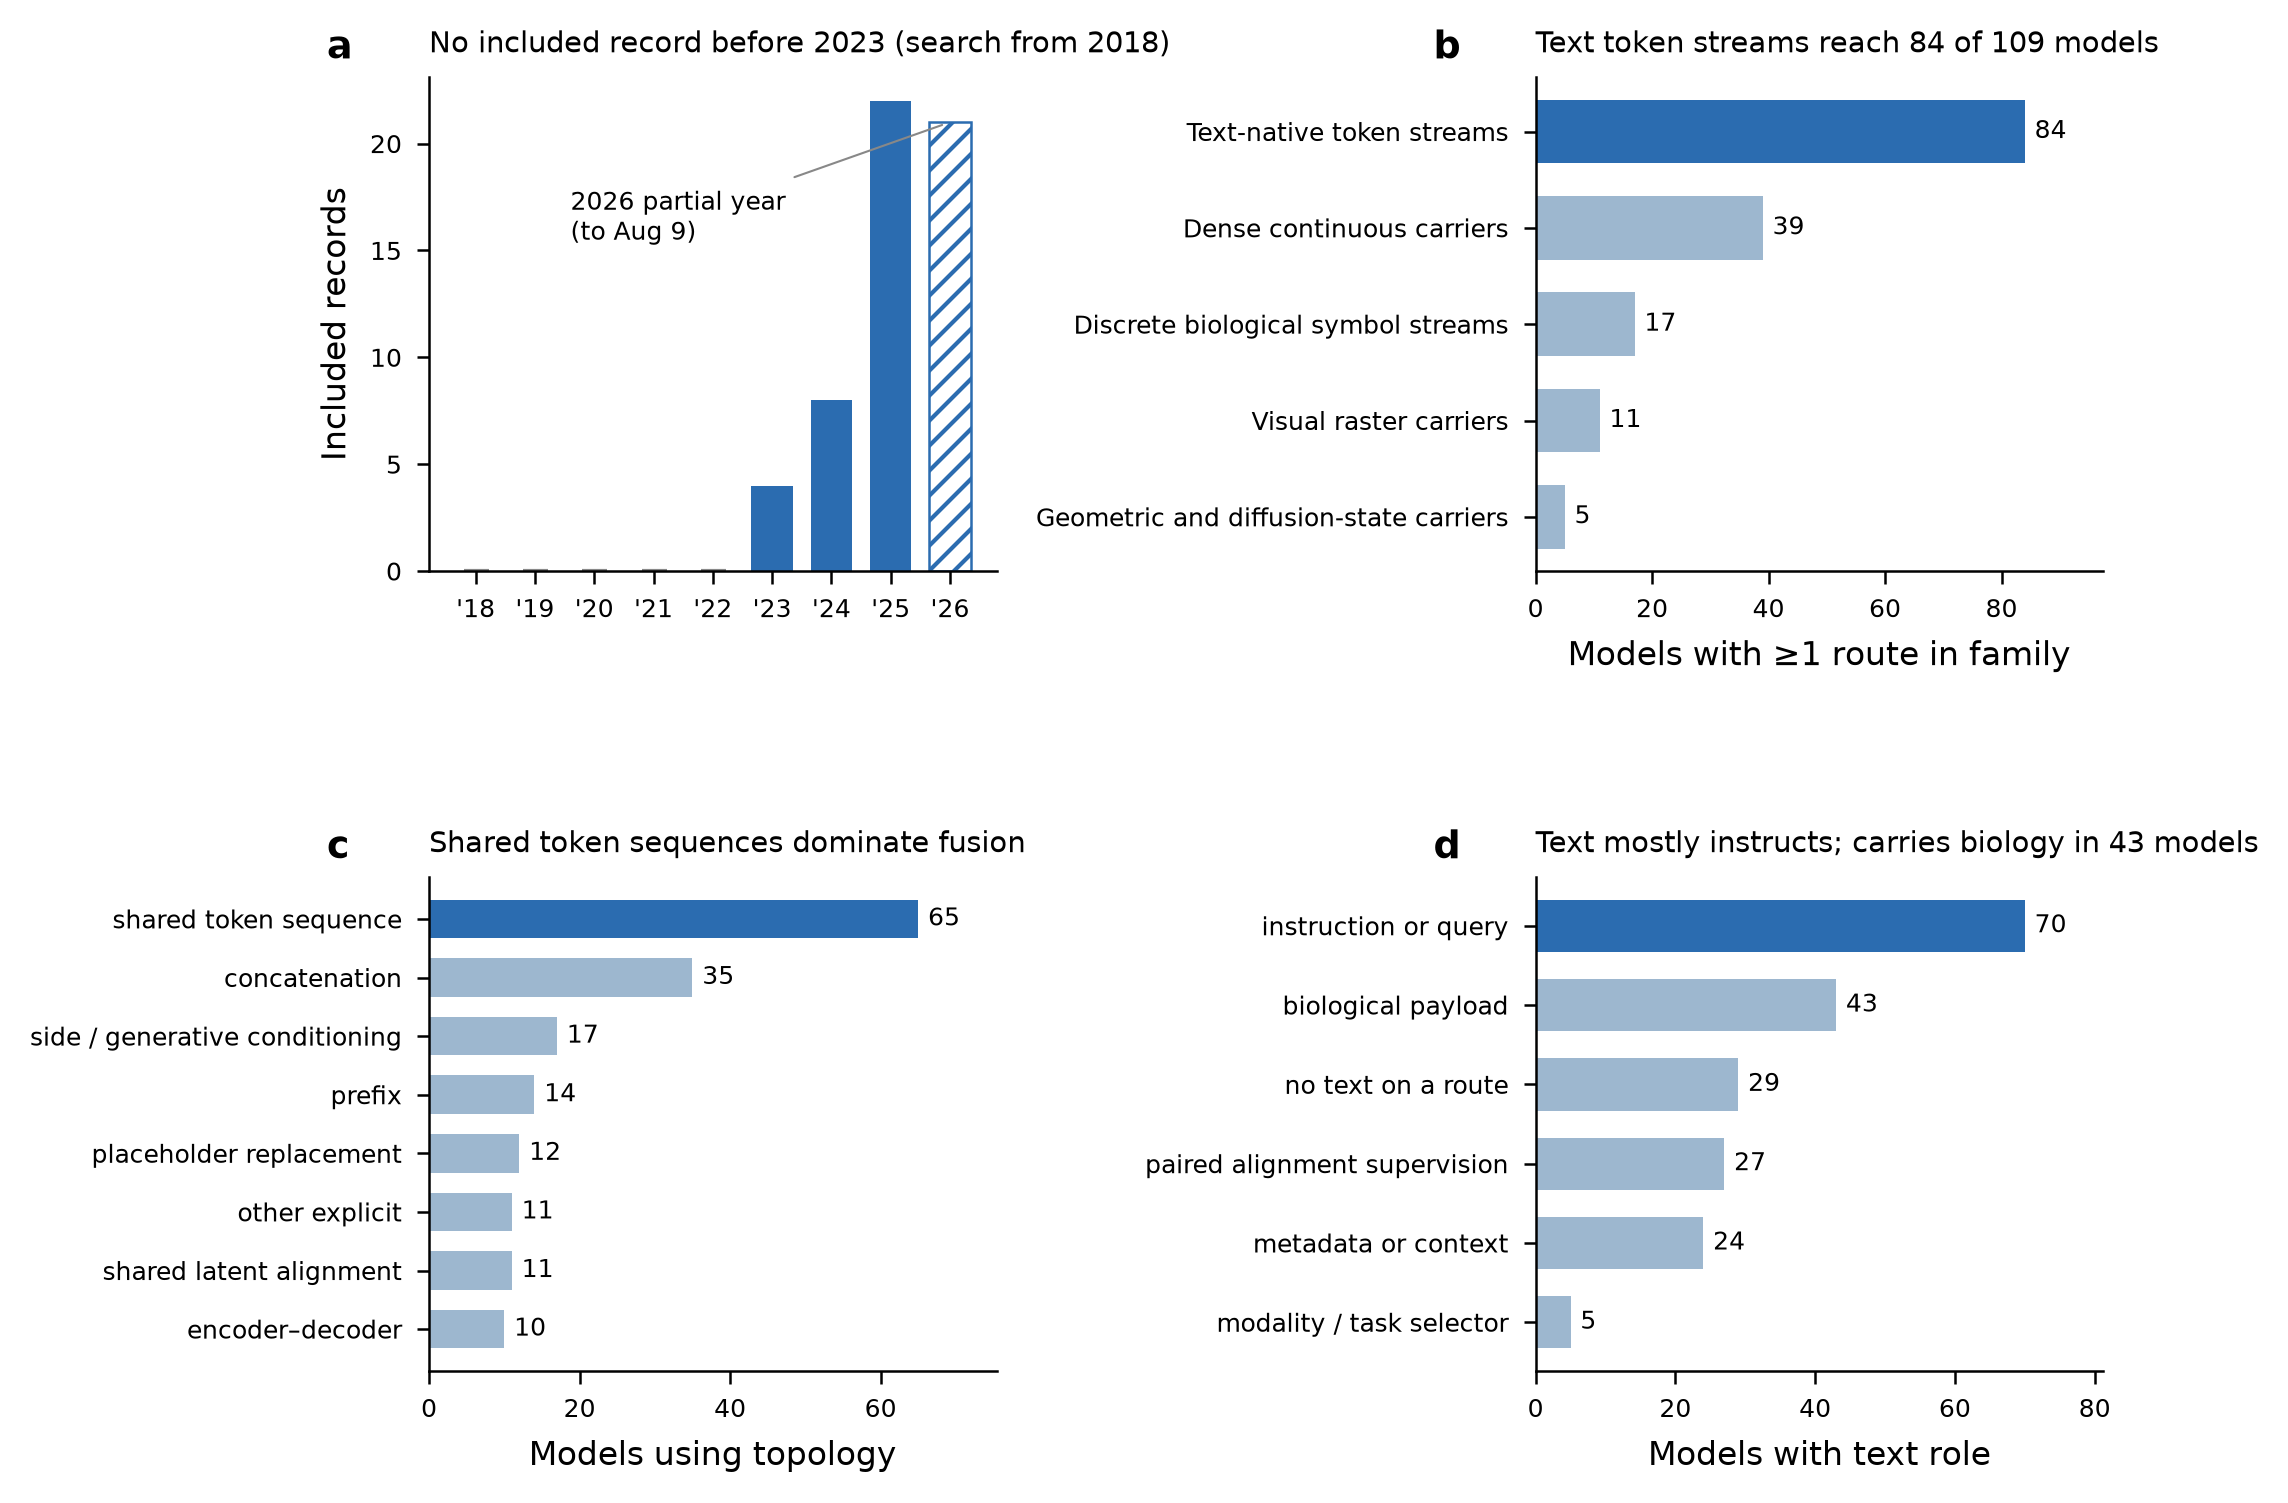
\includegraphics[width=\linewidth]{corpus_landscape.png}\end{minipage}
\caption{\textbf{Review flow and corpus.} Left: PRISMA 2020 flow with records identified per database (the same full flow is Supplementary Figure S1). Right: (a) included records per publication year, (b) models per input-carrier family, (c) fusion topology and (d) text role. \draftnote{Draft: the compact flow and the works-per-culture breakdown of panel a are still to be made; the panels shown are the current versions.}}\label{fig:2}
\end{figure*}


\subsection{Corpus characteristics (Figure 2b–d, Supplementary Table S1)}

\begin{itemize}
\item The 55 records describe 109 models (29 records describe one model; two describe eight), with 467 task/input configurations and 585 grounded routes.
\item After excluding the withdrawn OKR-Cell preprint, 54 records remain. Three studies have two reports each (Cell2Text, CellWhisperer, OmniNA), so the corpus contains 51 independent works. The culture-level analyses (\S{}3.4–3.10) count works, not records.
\item Publication years: 2023 (4), 2024 (8), 2025 (22), 2026 to 9 August (21). None from 2018–2022, although the search started in 2018. Years for 13 records added in 2026 top-ups come from the date-bounded search window.
\item Lifecycle phases charted: fine-tuning (53 models), evaluation (51), pretraining (38), inference (35).
\end{itemize}


\subsection{Operation-level input paths (Figure 3a–b)}

\textbf{Coverage.} We decomposed 54 papers: 4 author-curated pilot papers and 50 agent papers. The withdrawn OKR-Cell preprint is excluded. The decomposition yields 475 input paths, with 1,348 library-operation calls and 819 steps kept as unexpanded boundaries.

\begin{figure*}[!t]
\centering
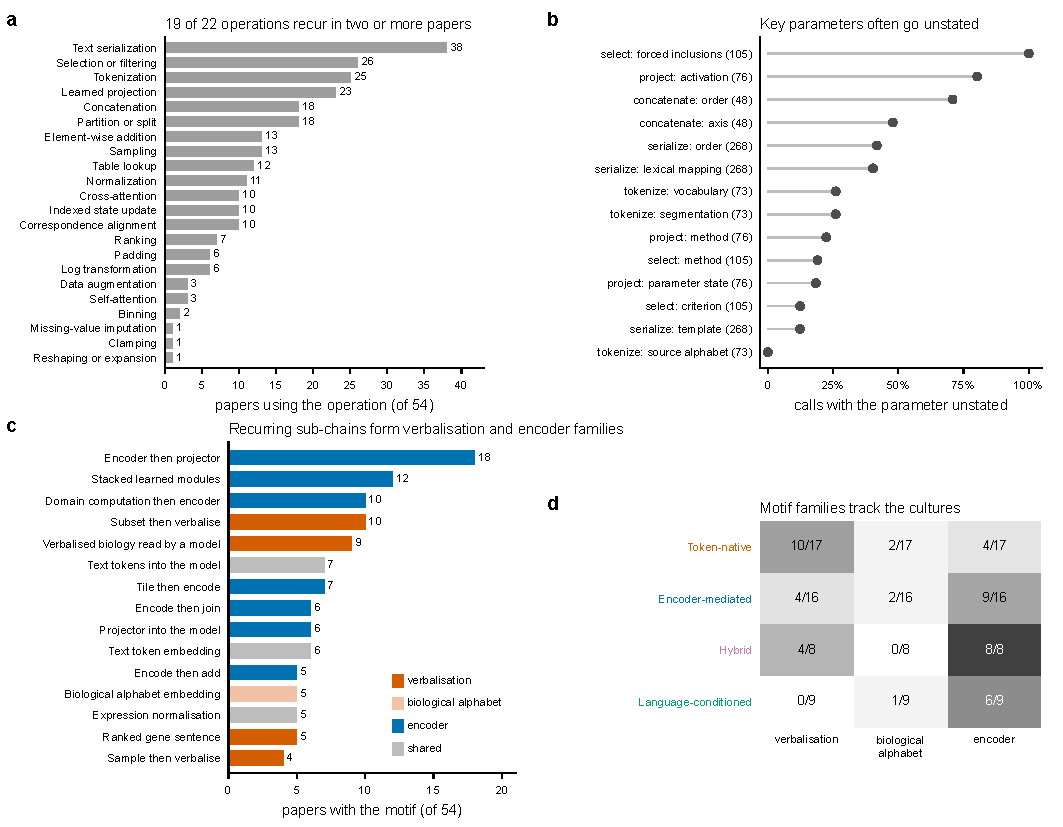
\includegraphics[width=\textwidth]{figure3.pdf}
\caption{\textbf{Input paths decompose into reusable operations and recurring motifs.} (a) Papers using each of the 22 library operations (release 1.3.0; 54 papers). (b) Share of calls whose parameter is not stated anywhere in the paper, for parameters with at least 45 calls (number of calls in parentheses; agent-decomposed papers). (c) The 15 motifs (closed frequent sub-chains supported by at least 4 papers), coloured by family: verbalisation (subset, rank or sample, then serialise; serialised biology read by a model), biological alphabet embedding, encoder (encoder, projector, stacked or joined learned modules), and shared text-handling or normalisation motifs. (d) Works in which a proposed or component model carries a motif of each family, by culture.}\label{fig:3}
\end{figure*}

\textbf{Consensus.} Of the 1,468 agent-decomposed steps, 1,394 (95.0\%) were decided identically in all three runs and 74 (5.0\%) by two of three; every step had a majority. Under v3.1 with frozen rules, the consensus of runs 1–3 and of runs 4–6 on ten unseen papers agreed on 95.6\% of steps and 85.4\% of complete routes. After the v3.2 boundary fixes, the same papers agree on 99.6\% and 98.8\%. That second figure is in-sample, because these papers informed the fixes. Across the three v3.2 production runs on all 50 agent papers, 90.9\% of route $\times$ run-pair comparisons had identical operation sequences (gate: at least 90\%) and the median paper-level operation-set Jaccard was 1.0, but five papers fell below the predeclared minimum of 0.75 (lowest 0.0 for Chroma, where one run produced a disjoint set). The full-corpus gate was therefore not met; release decisions use the per-step majority of the three runs (\nolinkurl{analysis/operation_decomposition_2026-10-07/stabilization/v32_all/stability.json}).

\textbf{Reuse.} 19 of the 22 operations occur in two or more papers. The most widespread are:

\begin{itemize}
\item text serialisation (38 papers);
\item selection (26);
\item tokenisation (25);
\item learned projection (23);
\item concatenation (18);
\item partition (18).
\end{itemize}

\textbf{Unexpanded steps.} In the median paper, 48\% of documented steps cannot be decomposed from the text (whole encoders, unstated fusion algebra, training mixtures).

\textbf{Unreported choices.} Of 2,433 parameter slots, 844 (35\%) are not stated anywhere in the paper; 88\% of slot decisions were unanimous across runs, and held-out consensus status agreement was 0.992. Among parameters with at least 45 calls, papers left unstated:

\begin{itemize}
\item the projection activation in 80\% of 76 calls;
\item the concatenation order in 71\% of 48;
\item the serialisation order in 42\% of 268;
\item the lexical rendering of values in 40\% of 268;
\item the token vocabulary in 26\% of 73.
\end{itemize}

Only 52 of the 262 biological routes with library calls (20\%) state every declared parameter, and only 4 of 43 works do so for all their biological routes.


\subsection{Two design cultures and a hybrid (Figures 1a and 3c–d)}

Biological routes fall into six main carrier $\times$ interface archetypes:

\begin{itemize}
\item encoded soft tokens (24 papers);
\item verbalised text in the token stream (18);
\item generator conditioning (17);
\item biological alphabets in the token stream (8);
\item attention bridges (7);
\item shared latent alignment (7).
\end{itemize}

The recurring operation sub-chains split along the same line. Verbalisation motifs (subset, rank or sample, then serialise) occur almost only in verbalised inputs. Encoder motifs (encoder then projector, stacked modules, encode-then-join) occur in the encoder-based archetypes. Of models whose motifs are all verbalisation motifs, 16 of 19 have a verbalised primary archetype; of models whose motifs are all encoder motifs, 23 of 28 have an encoder-based one. At the level of works, verbalisation motifs occur in 10 of 17 token-native and 4 of 16 encoder-mediated works, and encoder motifs in 9 of 16 encoder-mediated, 8 of 8 hybrid and 4 of 17 token-native works (Figure 3d). Culture follows the main route by which biology reaches the generative model (\S{}2.10), so a work can also carry motifs of the other family, for example in auxiliary routes or components.

At the level of works, this gives two cultures, a hybrid, and a separate family in which language conditions a biology model (Table 1):

\begin{table*}[!t]
\caption{Design cultures of the 51 independent works.}\label{tab:cultures}
\begin{tabularx}{\textwidth}{@{}>{\raggedright\arraybackslash}p{0.18\textwidth}>{\raggedright\arraybackslash}X r@{}}
\toprule
\textbf{Culture} & \textbf{Definition} & \textbf{Works} \\
\midrule
Token-native & biology written into the language model's own stream & 17 \\
Encoder-mediated & biology injected as encoder vectors & 16 \\
Hybrid & both channels in the same system & 8 \\
Language-conditioned & diffusion, flow, graph or sequence generators conditioned on text or text-derived embeddings & 9 \\
Alignment-only & no generative host & 1 \\
\botrule
\end{tabularx}
\end{table*}

The cultures are not dictated by the data. Transcriptomics is handled in every culture (token-native 9 works, encoder-mediated 8, hybrid 6, language-conditioned 7), and nucleotide sequences in both main ones (5 and 7). The operations that define each culture are near-universal within it:

\begin{itemize}
\item serialisation occurs in 94\% of works with verbalised routes;
\item tokenisation in 75\% of works with biological alphabets;
\item cross-attention in 71\% of works with attention bridges;
\item unexpanded learned modules in 57–100\% of works in the encoder-based archetypes.
\end{itemize}

\textbf{Why ``cultures''.} We use the term for a bundle of choices that travel together, not for the input route alone. Two parts of the bundle follow from the definition: what reaches the language model (\S{}3.5) and the motif families above, which are mined from the same routes. Two do not: the stated justifications, which describe the same trade-off from opposite sides (\S{}3.6), and the choice of opponents, which differs sharply by proposing culture (\S{}3.9). Other practices are shared: rates of LLM-written text, of dependence tests and of LoRA~\cite{lora} or full fine-tuning are similar in the two main cultures (\S{}3.7–3.8).


\subsection{What each culture keeps of the measurement (Figure 4)}

\textbf{Token-native routes keep identities and order and drop magnitudes.}

\begin{figure*}[!t]
\centering
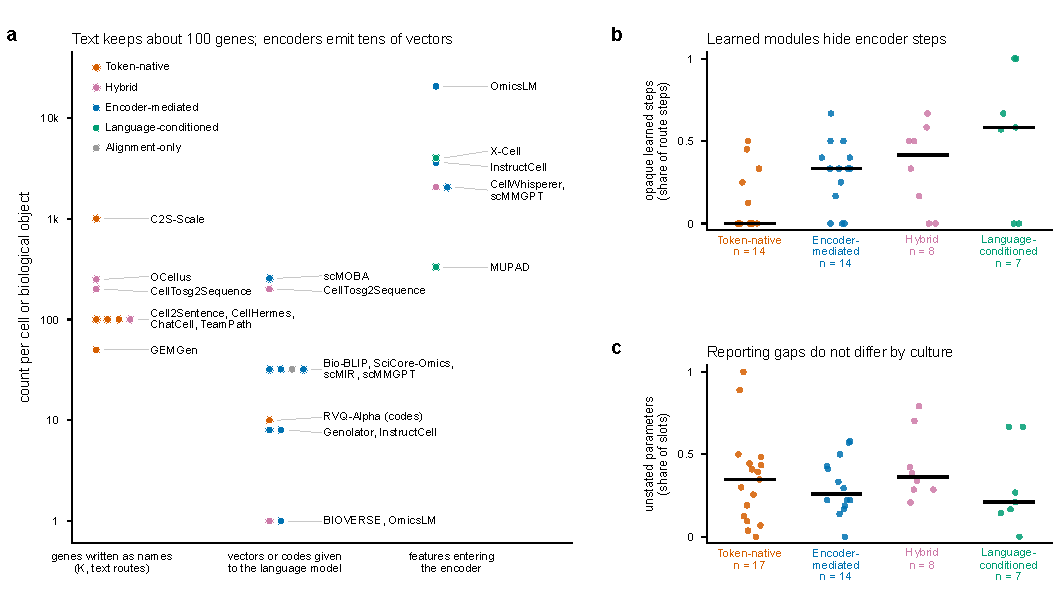
\includegraphics[width=\textwidth]{figure4.pdf}
\caption{\textbf{What each culture keeps of a measurement.} (a) Counts per cell or biological object as stated in the papers: genes kept when transcriptomes are written as names (proposed-model text routes; 8 works), vectors or discrete codes passed to the language model (11 works; RVQ-Alpha uses learned discrete codes in the token stream), and features entering the encoder (6 works). Points are works coloured by culture; works with the same value share a label. For comparison, Cell2Sentence reports about 350 text tokens for a prompt plus 100 genes. (b) Per-work median share of biological route steps that are opaque learned modules (works with agent-decomposed biological routes). (c) Per-work share of parameter slots unstated in the paper (proposed and component models; token-native vs encoder-mediated, Mann–Whitney p = 0.89). Bars are medians; the alignment-only work is omitted from b and c.}\label{fig:4}
\end{figure*}

\begin{itemize}
\item Works that write transcriptomes as text keep 50–1000 genes per cell, with a median of 100 over the 8 works that state K (\nolinkurl{gene_budget_table.csv}).
\item The genes are listed in rank order: Cell2Sentence~\cite{cell2sentence}, CellHermes~\cite{cellhermes}, ChatCell~\cite{chatcell} and TeamPath~\cite{teampath} keep 100, CellTosg2Sequence~\cite{celltosg2sequence} 200, and C2S-Scale~\cite{c2sscale} reports that 1000 often works well. OCellus'~\cite{ocellus} spatial prefix keeps 5 marker genes per neighbour.
\item Values are written as numbers in only 2 works (CpG beta values, blood-biomarker values).
\item Rank tie handling is never stated (0 of 24 ranking calls), and selection forced inclusions are stated in none of 105 selection calls.
\item Two works report that within-cell rank tracks log-expression (Cell2Sentence; CellTosg2Sequence, R$^{2}$ $\approx$ 0.90). If so, what a cell sentence cannot recover is mainly the genes outside the top K (at least 95\% of about 20,000 genes when K $\leq$ 1000), the order among ties, and any cell-specific departure from the population-level fit between rank and expression.
\end{itemize}

\textbf{Encoder routes pass magnitudes to learned modules and hide what survives.}

\begin{itemize}
\item Encoder routes in the six works that state their input size use 331–20,541 features (median about 2,800).
\item Eleven works with soft-token or query interfaces deliver each biological object to the downstream model as 1–256 vectors (median 32): 1 (BIOVERSE~\cite{bioverse}, OmicsLM~\cite{omicslm}), 8 (InstructCell, Genolator~\cite{genolator}), 10 discrete codes (RVQ-Alpha~\cite{rvqalpha}), 32 (scMMGPT~\cite{scmmgpt}, SciCore-Omics~\cite{scicoreomics}, Bio-BLIP~\cite{bioblip}, scMIR~\cite{scmir}), 200 (CellTosg2Sequence) and 256 (scMOBA~\cite{scmoba}) (\nolinkurl{token_budget_table.csv}).
\item For comparison, Cell2Sentence spends about 350 text tokens on a prompt plus 100 genes.
\item By culture, the counts above are: token-native works K = 50–1000 (5 works; hybrids 100–250, 3 works); encoder-mediated works 1–256 vectors (median 32, 7 works) from 2,048–20,541 features (3 works).
\item In the median encoder-mediated work, 0.33 of biological route steps are opaque learned modules, against 0 in the median token-native work. The projector activation is unstated in 82\% of encoder-projector motifs and the concatenation order in 95\% of encode-then-join motifs.
\end{itemize}

\textbf{Reporting completeness is similar in the two cultures.} The median share of unstated parameter slots per work is 0.35 in token-native and 0.26 in encoder-mediated works (Mann–Whitney p = 0.89). What differs is what is lost (measurement fidelity vs transparency of the transformation), not reporting discipline.


\subsection{How each culture justifies its choice (Figure 5a)}

Stated rationales were charted with verbatim evidence and adjudicated by the steward (rationale run agreement: mean Jaccard 0.60). The two cultures describe the same trade-off from opposite sides (Table 2).

\begin{figure*}[!t]
\centering
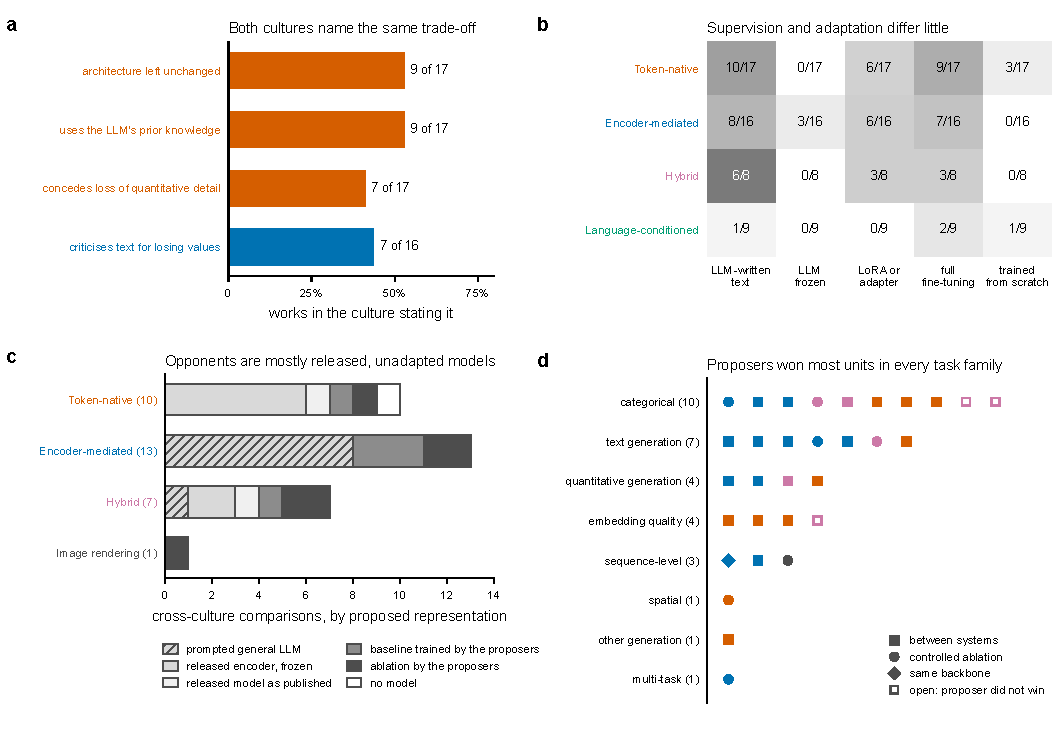
\includegraphics[width=\textwidth]{figure5.pdf}
\caption{\textbf{How the cultures justify and test their choice.} (a) Stated rationales, adjudicated from verbatim quotes: for the work's own representation (token-native works) or against text rendering (encoder-mediated works). (b) LLM-written text and adaptation of the language model by culture (cells: works / works in the culture; adaptation counted where both charting runs agree). (c) Opponent type in the 31 cross-culture comparison units, by proposed representation. (d) Units by task family; marker shape shows the design and colour the proposed culture; open markers are the three units the proposer did not win (two mixed, one loss). Contrasts between cultures are exploratory.}\label{fig:5}
\end{figure*}

\begin{table*}[!t]
\caption{Stated rationales for and against input representations, by culture (works; adjudicated from verbatim quotes).}\label{tab:rationales}
\begin{tabularx}{\textwidth}{@{}>{\raggedright\arraybackslash}p{0.2\textwidth}>{\raggedright\arraybackslash}X>{\raggedright\arraybackslash}X@{}}
\toprule
\textbf{Rationale} & \textbf{Token-native (of 17)} & \textbf{Encoder-mediated (of 16)} \\
\midrule
Unchanged architecture & 9 (e.g.\ C2S-Scale ``avoids modifying the underlying architecture of LLMs'') & none in both runs \\
Language model's prior knowledge of named entities & 9 & — \\
Concedes loss of quantitative or fine-grained information in its own representation & 7 (e.g.\ Cell2Sentence, CellHermes, ChatCell, RVQ-Alpha) & — \\
Criticises text rendering for losing magnitudes, low-abundance genes or structure & — & 7 (Cell2Text, BIOREASON~\cite{bioreason}, InstructCell, scMMGPT, scMOBA, Bio-BLIP, OmicsLM) \\
\botrule
\end{tabularx}
\end{table*}


\subsection{Supervision and adaptation (Figure 5b)}

\textbf{LLM-generated text.} 25 of 51 works (49\%) train or evaluate on text written or rewritten by another LLM (\nolinkurl{synthetic_text_table.csv}):

\begin{itemize}
\item in 20 works the generated text carries biological content (descriptions, captions, question–answer pairs, conversations, interpretations, reasoning traces); 4 generate only templates or instructions; 1 is unclear;
\item 7 works distill reasoning traces from frontier models;
\item 5 report a human check of the generated text;
\item in 4 works LLM-written text also enters the evaluation;
\item by culture: token-native 10 of 17, encoder-mediated 8 of 16, hybrid 6 of 8, language-conditioned 1 of 9.
\end{itemize}

Use of LLM-written text does not differ between the two main cultures (Fisher p = 0.73) and is rare only where language conditions a biology generator (1 of 9 vs 24 of 42 other works, p = 0.024). It is a property of language-model-hosted designs, not of either culture.

\textbf{Adaptation} (works where both runs agree):

\begin{itemize}
\item Token-native works fine-tune the language model fully (9) or with LoRA (6), train it from scratch (3), and extend its vocabulary (4).
\item Only encoder-mediated works keep the language model frozen (3 of 16, against 0 of 17 token-native works; Fisher p = 0.10). They freeze (6) or fine-tune (6) the biological encoder.
\end{itemize}


\subsection{Is the biology used? (Figure 1c)}

Twenty-two of 51 works (43\%) report any test of whether outputs depend on the biological input: removal, mismatch or shuffling, random input, a no-biology baseline, or content perturbation (run agreement: Jaccard 0.91; Table 3).

\begin{table}[!t]
\caption{Works reporting a test of whether outputs depend on the biological input, by culture.}\label{tab:dependence}
\begin{tabularx}{\columnwidth}{@{}>{\raggedright\arraybackslash}X r@{}}
\toprule
\textbf{Culture} & \textbf{Works with a dependence test} \\
\midrule
Token-native & 7 of 17 \\
Encoder-mediated & 4 of 16 \\
Hybrid & 5 of 8 \\
Language-conditioned & 6 of 9 \\
\botrule
\end{tabularx}
\end{table}

The rates do not differ detectably between cultures (encoder-mediated vs all other works, Fisher p = 0.13; token-native vs encoder-mediated, p = 0.46); the low overall rate is the finding. Bio-BLIP's authors argue that linear projection interfaces encourage reliance on prompt text, which would make such tests most informative for encoder-mediated designs. Works that made cross-culture comparisons tested dependence no more often than the others (10 of 20 vs 12 of 31, Fisher p = 0.56).

Evaluation formats (works, both runs / either run):

\begin{itemize}
\item closed-set classification 31 / 42;
\item open-text generation scored by automatic text metrics 29 / 43;
\item likelihood or perplexity scoring 9 / 13;
\item candidate-label selection 6 / 11;
\item open text judged by an LLM 6 / 7, or by humans 6 / 8;
\item wet-lab validation in 1 work.
\end{itemize}


\subsection{Head-to-head evidence between cultures (Figures 1b and 5c–d)}

The charting runs returned 217 comparison items. Adjudication merged them into 31 comparison units in 20 works whose arms belong to different cultures (\nolinkurl{comparison_units_adjudicated.csv}). Three further units were set aside as within-culture or not about representation form (\nolinkurl{comparison_units_removed.csv}).

\textbf{Home advantage.} The authors' own representation won 28 of 31 units:

\begin{itemize}
\item 20 of 23 between-system comparisons (87\%; two-sided binomial p = 4.9 $\times$ 10$^{-4}$ against 0.5);
\item all 7 controlled ablations;
\item the one same-backbone comparison.
\end{itemize}

Units are nested in works (C2S-Scale contributes four). Counted by work, the proposer won every unit in 17 of 20 works (sign test p = 0.0026) and every between-system unit in 14 of 17 (p = 0.013).

Across papers the winners split between cultures (between-system winners: token-native 10, encoder-mediated 9, hybrid 2, mixed 2), so no culture dominates. Within every task family the winner followed the proposer; the non-wins fell in categorical tasks (2 of 10 units) and embedding quality (1 of 4), and none in text generation (7 units), quantitative generation (4) or sequence-level tasks (3).

\textbf{Each culture tests mostly against released, unadapted forms of the other.}

\begin{itemize}
\item In encoder papers, the opponent was a prompted general LLM reading raw text in 8 of 13 units: GPT-4.1, GPT-4o~\cite{gpt4o} or Llama-2-Chat~\cite{llama2} given sequences, SMILES or gene lists without adaptation.
\item In token-native papers, it was a released encoder-based model in 7 of 10 units, usually a frozen embedding with a simple head (scGPT~\cite{scgpt}, Geneformer~\cite{geneformer}, ESM-2~\cite{esm2}, Nicheformer~\cite{nicheformer}) or a model used as published (CellWhisperer).
\item The opponent type differs sharply by proposing culture (prompted LLMs 8 of 13 vs 0 of 10, Fisher p = 0.003; released encoder models 0 of 13 vs 7 of 10, p = 4.9 $\times$ 10$^{-4}$). This is partly by construction, since a cross-culture opponent must come from the other culture; the choice of an unadapted opponent is not.
\item Opponents trained by the proposing team on the same data (baselines or ablations) made up 5 of 13 units in encoder papers and 2 of 10 in token-native papers. Across all cultures the proposer won all 11 such units and 16 of 19 units against released opponents; the remaining unit compared representations without a model. All three exceptions involved released opponents.
\end{itemize}

\textbf{What the comparisons show.}

\begin{itemize}
\item When the token-native arm read raw sequence letters, the encoder arm won 5 of 7 units. The exceptions were a rendering of DNA as images (OpticalDNA~\cite{opticaldna}) and a vocabulary trained on biological tokens (OmniGene-4~\cite{omnigene4}).
\item For gene-name lists, the winner followed the proposing culture (token-native 8, encoder-mediated 7, hybrid 3, mixed 2).
\item The three exceptions:
\begin{itemize}
\item a 120B general model reading 128 gene names beat the 8B hybrid BIOVERSE on zero-shot annotation (accuracy 0.779 vs 0.614), while an 8B general model did not (0.369);
\item C2S-Scale-27B beat the 32B hybrid CellTosg2Sequence on immune annotation (exact 85.6\% vs 24.1\%); the CellTosg2Sequence authors attribute the gap to C2S-Scale's much larger pretraining corpus, against about 8,000 annotation examples in their own reinforcement stage;
\item OCellus embeddings won a linear probe but not clustering.
\end{itemize}
\item In controlled ablations, where only the representation changed, the encoder or hybrid arm won whenever the authors had proposed it:
\begin{itemize}
\item expression values vs cell sentences in scMMGPT (annotation error 0.76\% vs 6.42\%);
\item aligned features vs a raw sequence in the same Llama-2-Chat (BioMedGPT; BLEU-2 0.344 vs 0.019);
\item an embedding stack vs a Cell2Sentence-like control (OmicsLM; average relative rank .740 vs .090).
\end{itemize}
\item The token-native arm won the one controlled test its authors proposed: numeric coordinate tokens vs learned positional embeddings in TISSUENARRATOR~\cite{tissuenarrator}, reported qualitatively.
\end{itemize}


\subsection{Hybrids and change over time}

Eight works combine both channels, and 11 deliver one modality through two carrier formations. In both controlled tests the hybrid beat its single channel:

\begin{itemize}
\item CellWhisperer: an embedding plus the top-50 gene list, a mild benefit;
\item CellTosg2Sequence: knowledge-graph tokens plus a cell sentence, 0.385 vs 0.268 fuzzy accuracy.
\end{itemize}

In both cases the hybrid was the proposed configuration. A related within-culture result points the same way: in RVQ-Alpha, adding gene evidence in text to learned discrete codes gained 8.3 percentage points and reduced hallucinations. Hybrids appear from 2024 on (1, 4 and 3 works in 2024–2026).

Soft tokens are the most or jointly most frequent archetype in every year. The share of papers using verbalisation was 38\% in 2024 and 50\% in 2026, and biological alphabets rose from 0\% to 28\%. Yearly counts are small (4, 8, 20 and 18 papers).


\section{Discussion}


\subsection{Principal findings}

Generative text–omics foundation models are built in two design cultures:

\begin{itemize}
\item \textbf{translating} biology into the language model's own tokens;
\item \textbf{encoding} it with biological models and injecting vectors.
\end{itemize}

A growing hybrid combines both, and a separate family uses language to condition biology models. The cultures are not imposed by the data: transcriptomes and sequences are handled both ways.

The cultures keep complementary parts of a measurement:

\begin{itemize}
\item Token-native inputs keep identities and order, and lose explicit values and every gene outside the top K.
\item Encoder-mediated inputs pass values and structure to learned modules, so what survives is not visible and is rarely tested.
\end{itemize}

Where authors discuss the choice, they describe this trade-off the same way from both sides: token-native works cite unchanged architectures and the language model's knowledge of named entities and concede the loss of quantitative information, while encoder-mediated works criticise text rendering for that loss. The distinction itself is familiar. What has been missing is a measurement of its consequences and evidence about when each side of the trade-off matters.


\subsection{Why the published comparisons cannot settle the question}

Three features of the evidence keep it from discriminating between cultures.

\begin{enumerate}
\item \textbf{Home advantage.} The proposing culture won 28 of 31 cross-culture comparisons (every comparison in 17 of 20 works), including every controlled ablation. Selective publication alone would produce this pattern, so these wins cannot rank the cultures.
\item \textbf{Unadapted opponents.} Each culture tests mostly against released, unadapted forms of the other:
\begin{itemize}
\item encoder papers against general LLMs that read raw sequences or gene lists without adaptation;
\item token-native papers against released encoder models, usually frozen embeddings with simple heads.
\end{itemize}
When both arms are trained on the same data, the comparison is an ablation or baseline built by the proposers, who also decide what to ablate; the proposer won all 11 such units.
\item \textbf{Rare dependence tests.} Only 22 of 51 works test whether outputs depend on the biological input, with no detectable difference between cultures. Without such tests, a win cannot be attributed to the representation rather than to prompt text, metadata or the language model's prior knowledge.
\end{enumerate}

The few results that went against the proposer are informative. They suggest that verbalised gene lists can be competitive for categorical identity tasks such as cell annotation when the reading model is large or trained on a great deal of single-cell data. Encoders won most units (5 of 7) in which the text arm had to read raw sequence letters. These are hypotheses for a controlled study, not conclusions.


\subsection{A neutral comparison protocol (Box 1)}

We propose that claims about input representation be supported by comparisons that fix everything except the representation (Box 1).


\subsection{A reporting card for input representations (Box 1)}

Reporting completeness is similar across cultures, but the missing items differ (Box 1).

\begin{boxtext}[A neutral comparison protocol and a reporting card for input representations]
\textbf{Neutral comparison protocol} (everything fixed except the representation)
\begin{itemize}
\item \textbf{Matched systems:} the same backbone, data, training budget and adaptation (LoRA or full fine-tuning) for every arm.
\item \textbf{Matched information budget:} report the features kept and the tokens per object for each arm, and vary K for verbalised arms.
\item \textbf{Tasks at both levels:} identity-level tasks (annotation, retrieval) and magnitude-level tasks (perturbation response, expression or dose prediction, variant effect).
\item \textbf{Dependence controls:} removal, mismatch and shuffling of the biological input, plus a no-biology baseline with the same backbone; for verbalised inputs, also gene-name scrambling.
\item \textbf{Like-for-like baselines:} when a published method is used as a comparator, use its documented settings (for example the number of genes in a cell sentence), or report both.
\end{itemize}

\textbf{Reporting card.} Items to report for each input representation:

\noindent\begin{tabularx}{\linewidth}{@{}>{\raggedright\arraybackslash}p{0.3\linewidth}>{\raggedright\arraybackslash}X@{}}
\toprule
\textbf{Culture} & \textbf{Card items} \\
\midrule
Token-native & K, selection criterion, ordering and tie rule, normalisation, template, lexical rendering of values, vocabulary or segmentation \\
Encoder-mediated & encoder and its training state, projector method and activation, number of vectors per object, which components are trained, concatenation order and axis \\
LLM-generated supervision (all cultures) & generator and version, prompts, decoding parameters, verification \\
\botrule
\end{tabularx}

Operation library 1.3.0 provides a controlled vocabulary for these items.
\end{boxtext}


\subsection{Relation to existing reviews}

Recent surveys classify models by family, modality and task; LLM4Cell~\cite{llm4cell}, for example, groups 58 single-cell methods into five methodological families and maps them to eight analytical tasks. \citeplaceholder{CITE, to verify: ACL 2025 survey of single-cell foundation language models; LLMs meet virtual cell; Nature 2025 perspective on multimodal foundation models in molecular cell biology; 2026 Cell Systems compositional-FM review; scoping review of LLM-generated synthetic data in biomedicine.} The translate-or-encode distinction is familiar to primary authors, who use it to justify their designs (\S{}3.6). This review measures, at the level of operations, what each design keeps and how its claims are tested, across omics modalities.


\subsection{Implications}

For builders, the current evidence supports working hypotheses rather than rules:

\begin{itemize}
\item identity-level tasks may be served by verbalised inputs read by strong language models;
\item tasks that depend on magnitudes or raw sequence may favour encoders;
\item hybrids beat their single channels in both controlled tests, both run by their proposers.
\end{itemize}

Each hypothesis can be tested with the protocol in Box 1.

For reviewers and benchmark designers, the priority is neutral, budget-matched comparisons with dependence controls, rather than further between-system leaderboards.


\section{Limitations}

\begin{itemize}
\item LLM-assisted screening, charting and decomposition; the decomposition used \nolinkurl{gpt-5.6-luna} because the earlier \nolinkurl{gpt-5.4-mini} is no longer served through Codex. Agent graphs are three-run consensus decisions, not author-verified reconstructions, and were not checked by a reviewer agent.
\item Decomposition stability is incomplete. On unseen papers, the step-level consensus was reproduced in 95.6\% of steps but complete route sequences only in 85.4\%, below the predeclared 90\% gate. Among the three production runs on all 50 agent papers, five papers had a pairwise operation-set Jaccard below the predeclared minimum of 0.75 (one at 0.0), so the full-corpus gate was not met either. Residual disagreement concerns how prompts are merged with metadata (serialisation vs concatenation) and whether a named ``tokenized'' representation counts as a tokenisation step. The rules were tuned on development and earlier held-out papers, so in-sample stability is higher than out-of-sample stability. Steps are bounded by the charted routes, so errors in charting carry over.
\item Parameter status was decided by agents, not authors. Held-out consensus agreement was high (0.992), but single-run agreement on the 30 papers outside the development and held-out sets was lower (0.912 vs 0.956 held-out), and one run needed a clean restart after a quote failed validation. ``Unstated'' means not found in the paper text; values in code or cited works are not credited.
\item LLM-assisted screening and charting; stability is reported separately. Role-separated prompts are not independent reviewers.
\item Open access and English were required. At search they were applied only in PubMed (with ``free full text'' as a proxy for open access), Scopus and OpenAlex, and elsewhere at screening. 15 reports could not be retrieved and 14 had no valid targeted section pair.
\item Google Scholar was incomplete in three rounds (5 of 7 queries in April and June, no records in July). One eligible record was found only after a recall correction.
\item The executed search windows have a 13-day gap.
\begin{itemize}
\item The baseline was run on 2026-02-15 with a window to 2026-02-28, and the first top-up started at 2026-03-01. The date-bounded sources were therefore never queried for records dated 2026-02-16 to 2026-02-28.
\item Two routes reached part of this window: Google Scholar's year-level queries in later rounds, and dates that differ between databases.
\item On 2026-10-14 we re-ran the baseline queries of PubMed, arXiv, Europe PMC and Semantic Scholar for the window. They returned 51 unique records. 17 had already been retrieved and 34 had not; none of the 34 met the eligibility criteria in an indicative single-pass LLM title/abstract triage.
\item Scopus and Springer Nature were not re-run (\nolinkurl{analysis/prisma_search_audit_2026-10-14/}).
\end{itemize}
\item The search vocabulary covered omics data only (\S{}2.2).
\begin{itemize}
\item A coverage check found that 12 protein and biomolecular text–generative models (ProteinDT~\cite{proteindt}, BioT5~\cite{biot5}, BioT5+~\cite{biot5plus}, NatureLM~\cite{naturelm}, Evolla~\cite{evolla}, Galactica~\cite{galactica}, InstructProtein~\cite{instructprotein}, ProtLLM~\cite{protllm}, Prot2Text~\cite{prot2text}, ProtT3~\cite{prott3}, ProLLaMA~\cite{prollama}, TxGemma~\cite{txgemma}) were never retrieved. None has a term of the biological-data block in its title or abstract.
\item In the PubMed query for 2018-01-01 to 2026-08-09, a protein block in place of the biological-data block adds 1,140 records that the original block does not match (the original query returns 939), and a nucleotide block adds 508. In Europe PMC preprints the additions are 1,130 and 633 (hit counts on 2026-10-15).
\item The findings therefore describe omics-framed models. Models whose only biological input is a protein are represented by three works (\S{}2.2), and nucleotide-sequence models described without omics terms are under-represented. Whether the two cultures and the home advantage hold for these families is untested (Supplementary Text S2).
\end{itemize}
\item In the baseline full-text screening (2026-07-10), the abstract shown with the selected sections was cut to about 1,500 characters for 73 of 221 records (selected sections were complete), and five reports whose only reconstructed section covered at least 90\% of the paper were not screened at full text. The author judged the risk of missed inclusions low and kept the included set (\nolinkurl{analysis/length_truncation_audit_2026-10-09.md}).
\item The withdrawn OKR-Cell preprint is still counted in the 55 records (author decision pending).
\item Search closed on 2026-08-09; no refresh was done for this manuscript.
\item Motifs are mined from route chains bounded by the charted transformation chains and from four author-curated pilot graphs, so steps that the charting did not record cannot form motifs. Support thresholds (at least 4 papers) and motif naming involved author judgement.
\item The design-pattern axes are derived from the charted routes and their decomposition. Interface and carrier labels inherit charting errors, and A3 falls back on the charted carrier subtype for 90 biological routes whose chain has no decided operation. The axes were defined by the authors after inspecting the data and were not validated on an independent corpus.
\item Protocol objective 3 (datasets, downstream tasks, evaluation metrics) and the extraction fields for pretraining objective and code/data availability are not yet charted, except the evaluation formats and outputs recorded in the targeted pass (\S{}2.11).
\item The design-culture analysis (\S{}2.10–2.11) was defined after exploring the decomposed corpus, so its hypotheses are post hoc. Its charting used two runs of one model family and adjudication by a single steward. Run agreement was high for comparison presence ($\kappa$ 0.92), LLM-generated text ($\kappa$ 0.96) and dependence tests (Jaccard 0.91), but lower for evaluation formats (0.57) and rationales (0.60). A second human coder for the 31 comparison units and the culture assignment is planned before submission.
\item Culture assignment for works that combine separate models is a judgement call. Geneverse~\cite{geneverse} is coded token-native, although its image models are encoder-mediated.
\item Group sizes are small (17, 16, 8 and 9 works), and culture contrasts are exploratory (unadjusted Fisher tests). Comparisons are as reported by the authors; publication bias contributes to home advantage, so it is part of the finding as well as a limitation.
\item Comparisons reported only in figures can be missed by the charting runs. While checking one exception (CellTosg2Sequence), we found a Tahoe-100M~\cite{tahoe100m} perturbation-classification comparison against C2S-Scale-27B, won by the proposer, that neither run charted; it is not counted. Such misses would add to home advantage. The second-coder check will include a recall audit of comparisons.
\item Gene and token budgets are taken from stated values in 8 and 11 works; works that do not state them are not counted.
\item Earlier keyword pre-screens of the full texts (used to choose the variables for the targeted pass) skipped appendices after the reference list. All reported counts come from the targeted pass, which used the complete text.
\end{itemize}


\section*{Key Points}
\begin{itemize}
\item Generative text--omics foundation models follow two design cultures: token-native models write biology into the language model's own tokens, and encoder-mediated models inject vectors from biological encoders; hybrids combine both.
\item Token-native inputs keep gene identities and their order (a median of 100 genes per cell) and rarely keep measured values; encoder-mediated inputs pass values to learned modules whose transformation is not visible.
\item Only 22 of 51 works test whether outputs depend on the biological input, and 25 train or evaluate on text written by another LLM.
\item The proposing team's representation won 28 of 31 cross-culture comparisons, mostly against released, unadapted opponents, so the published evidence cannot rank the two cultures.
\item A neutral comparison protocol (matched systems and information budgets, identity- and magnitude-level tasks, dependence controls) and a reporting card for input representations are proposed (Box 1).
\end{itemize}

\section*{Supplementary data}
Supplementary data are available in the project repository (paths below).
% Generated by scripts/build_manuscript_latex.py; do not edit.
\begin{itemize}
\item Supplementary Figure S1. Full PRISMA 2020 flow, with records identified per database (\nolinkurl{analysis/prisma_flow_2026-10-07/prisma_flow.png}).
\item Table S0. Search runs by round and database: interface, execution date, limits as executed, records returned and retained (\nolinkurl{analysis/prisma_search_audit_2026-10-14/search_runs_by_database.csv}).
\item Text S1. Search strategies as executed (\nolinkurl{analysis/prisma_search_audit_2026-10-14/search_strategies_as_executed.md}), with the PRISMA-S audit and the coverage check of 2026-02-16 to 2026-02-28 (\nolinkurl{PRISMA_S_AUDIT.md}, \nolinkurl{gap_probe_2026-02-16_28.json}, \nolinkurl{gap_probe_indicative_triage.json}).
\item Text S2. Coverage check for protein and biomolecular text–generative models and the size of the vocabulary gap (\nolinkurl{analysis/prisma_search_audit_2026-10-14/protein_text_models_coverage_check.md}).
\item Table S1. Per-model charting table (\nolinkurl{analysis/review_synthesis_2026-10-07/charting_table_models.csv}).
\item Table S2. Full-text exclusions with reasons (\nolinkurl{analysis/prisma_flow_2026-10-07/PRISMA_FLOW.md}).
\item Table S3. Library steward queue (\nolinkurl{analysis/operation_decomposition_v32_2026-10-14/STEWARD_QUEUE.md}).
\item Table S4. Route-level design-pattern codebook (\nolinkurl{analysis/design_taxonomy_2026-10-13/taxonomy_codebook.csv}).
\item Table S5. Motif library (\nolinkurl{analysis/motif_library_2026-10-14/MOTIF_LIBRARY.md}, \nolinkurl{motifs.json}).
\item Table S6. Work-level culture assignment and charted variables (\nolinkurl{analysis/design_culture_charting_2026-10-14/v11/work_culture_table.csv}, \nolinkurl{steward_adjudication.json}).
\item Table S7. Cross-culture comparison units (\nolinkurl{analysis/design_culture_charting_2026-10-14/v11/comparison_units_adjudicated.csv}).
\item Table S8. Gene and token budgets, and LLM-generated text (\nolinkurl{analysis/discovery_2026-10-14/gene_budget_table.csv}, \nolinkurl{token_budget_table.csv}, \nolinkurl{synthetic_text_table.csv}).
\end{itemize}


\section*{Data availability}
The search configurations, screening and charting outputs, the operation library (release 1.3.0), the analysis code and the source data of every figure panel are available at \url{https://github.com/BogdanDidenko/text-bio-fundational-models-review}. The component library is browsable at \url{https://bogdandidenko.github.io/text-bio-fundational-models-review/component-library/}. An archived snapshot will be deposited at Zenodo \todo{DOI to be added}.

\section*{Use of large language models}
Screening, charting and operation-level decomposition used large language model agents, as described in Methods (Sections 2.5--2.11), with the prompts, schemas and run logs in the repository. \todo{The authors state here any use of language models in drafting or editing this manuscript, as required by the journal's policy.}

\section*{Funding}
\todo{Funding statement.}

\section*{Conflict of interest}
\todo{Competing interests statement, confirmed by all authors.}

\section*{Author contributions}
\todo{Contributions of each author, by initials.}

\section*{Acknowledgements}
\todo{Acknowledgements.}

\bibliographystyle{vancouver-draft}  % local copy of vancouver.bst, see its header
\bibliography{references}

\begin{biography}{}{\author{Bogdan Didenko} \todo{Position, affiliation and research interests (one or two sentences).}}
\end{biography}

\begin{biography}{}{\author{\todo{Co-author}} \todo{Biographical note.}}
\end{biography}

\end{document}
